\documentclass[class=report,crop=false, 12pt]{standalone}
\usepackage[screen]{../scratch}

\begin{document}


\titre[E]{Entrée/Sortie}
%===============================


\begin{enigme}

Pour ce programme, Scratch termine en disant \og $28118$ \fg{}.

\begin{center}
  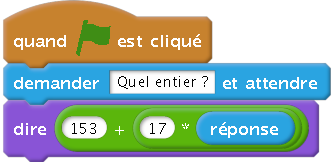
\includegraphics[scale=\scalebloc]{bloc-05-eg1} 
\end{center}


\bigskip

\textbf{Question.} Quel entier l'utilisateur a t-il saisi en entrée ?

\bigskip

\textbf{Bonus.} Quelle machine a été inventée cette année-là ?

%\begin{solution}
%$1645$, date de création de la pascaline.
%\end{solution}

\end{enigme}



\begin{enigme}

Pour dessiner ce chiffre \og 4 \fg{}, j'ai donné à Scratch une suite d'instructions en tapant des lettres au clavier.

\myfigure{0.7}{
\tiny  \tikzinput{figure-05-eg2}
} 

Voici comment Scratch réagit lorsqu'une touche est tapée : 
\begin{itemize}
  \item la touche \mot{h} ajoute $60$ à $x$,
  \item la touche \mot{p} retire $100$ à $x$,
  \item la touche \mot{y} ajoute $110$ à $y$,
  \item la touche \mot{n} retire $170$ à $y$,  
  \item la touche \mot{o} place le stylo en position d'écriture,
  \item la touche \mot{t} relève le stylo.  
\end{itemize}

\bigskip

\emph{Indications.}
\begin{itemize}
  \item Comme d'habitude Scratch part de $(0,0)$ orienté vers la droite, stylo en position d'écriture.
  
  \item Il est important de faire patienter Scratch (par exemple $0.2$ seconde) après avoir exécuté une instruction
  (pour éviter la répétition involontaire des touches tapées).
   
\end{itemize}

\bigskip

\textbf{Question.} Quelle suite de lettres ai-je tapée au clavier ?
Donner la réponse sous forme d'un mot.


%\begin{solution}
%\og \mot{python} \fg{} : un langage informatique moderne et puissant.
%\end{solution}

\end{enigme}



\begin{enigme}
Pour dessiner ce parcours, je donne à Scratch des instructions en tapant au clavier 
les lettres suivantes :

\centerline{\mot{b c a b s b b i b c i b}}

\myfigure{0.8}{
\footnotesize  \tikzinput{figure-05-eg3}
} 

À chacune des cinq lettres : \mot{a b c i s} correspond une instruction.

Le problème est que j'ai oublié la correspondance entre les lettres et les instructions que voici :
\begin{itemize}
  \item une première lettre fait avancer Scratch de $50$,
  \item une deuxième lettre fait tourner Scratch de $30$\textdegree\ vers la droite,  
  \item une troisième lettre fait tourner Scratch de $30$\textdegree\ vers la gauche,  
  \item une quatrième lettre fait tourner Scratch de $60$\textdegree\ vers la droite,   
  \item une cinquième lettre augmente la taille du stylo.  
\end{itemize}

\bigskip

\emph{Indications.}
Encore une fois, Scratch part de $(0,0)$, est orienté vers la droite ($90$\textdegree), stylo en position d'écriture.


Quelle est la première lettre (parmi \mot{a}, \mot{b}, \mot{c}, \mot{i}, \mot{s}),
puis la deuxième... ? %(parmi les mêmes touches)

\textbf{Question.} Quel mot (anglais) de cinq lettres est formé en juxtaposant ces cinq lettres ?


%\begin{solution}
%\og \mot{basic} \fg{} : un ancien langage informatique facile à apprendre.
%\end{solution}


\end{enigme}



\end{document}

